% Source: graduate-coursework/Research/Intro_to_Agents/slides/From_LLMs_to_Multi_Agent_Systems_slides.tex

\documentclass[border=4pt]{standalone}
\usepackage[T1]{fontenc}
\usepackage{graphicx}
\usepackage{tikz}
\usepackage{xcolor}
\usetikzlibrary{arrows.meta,positioning,shapes.geometric,fit,calc,
                decorations.pathreplacing,backgrounds,patterns,trees}

\definecolor{garnet}{HTML}{73000A}
\definecolor{rose}{HTML}{CC2E40}
\definecolor{atlantic}{HTML}{466A9F}
\definecolor{congaree}{HTML}{1F414D}
\definecolor{horseshoe}{HTML}{65780B}
\definecolor{grass}{HTML}{CED318}
\definecolor{honeycomb}{HTML}{A49137}
\definecolor{warmgrey}{HTML}{676156}
\definecolor{sandstorm}{HTML}{FFF2E3}
\definecolor{bk90}{HTML}{363636}
\definecolor{bk70}{HTML}{5C5C5C}
\definecolor{bk50}{HTML}{A2A2A2}
\definecolor{bk30}{HTML}{C7C7C7}
\definecolor{bk10}{HTML}{ECECEC}

\tikzset{
  agentbox/.style={
    rectangle, draw=#1, fill=#1!8, thick,
    minimum width=2.2cm, minimum height=0.8cm,
    font=\small\sffamily, align=center,
    inner sep=4pt
  },
  agentbox/.default=garnet,
  workerbox/.style={
    rectangle, draw=atlantic, fill=atlantic!8, thick,
    minimum width=1.8cm, minimum height=0.7cm,
    font=\small\sffamily, align=center,
    inner sep=3pt
  },
  tierbox/.style={
    rectangle, draw=#1, fill=#1!5, thick,
    minimum width=6.5cm, minimum height=1.0cm,
    font=\small\sffamily, align=center,
    inner sep=4pt
  },
  tierbox/.default=garnet,
  dataarrow/.style={
    -{Stealth[length=5pt]}, thick, color=#1
  },
  dataarrow/.default=bk70,
  brace/.style={
    decorate, decoration={brace, amplitude=6pt, raise=2pt}, thick, color=#1
  },
  brace/.default=bk50,
  labelnode/.style={
    font=\scriptsize\sffamily, color=bk70
  },
  codebox/.style={rectangle, draw=bk70, fill=bk90, text=white,
    font=\ttfamily\small, inner sep=6pt, align=left, text width=#1},
  codebox/.default=6cm,
  sysprompt/.style={rectangle, draw=rose, dashed, fill=rose!5, thick,
    minimum width=2.0cm, minimum height=0.6cm,
    font=\small\sffamily, align=center, inner sep=3pt},
  tooldef/.style={rectangle, draw=atlantic, fill=atlantic!8, thick,
    minimum width=1.8cm, minimum height=0.6cm,
    font=\small\sffamily, align=center, inner sep=3pt},
  wrapperbox/.style={rectangle, draw=garnet, dashed, thick, fill=garnet!3,
    inner sep=8pt},
  pbar/.style={rectangle, draw=#1, fill=#1!30, thick,
    minimum height=0.3cm, font=\scriptsize\sffamily},
  pbar/.default=horseshoe,
  flag/.style={rectangle, draw=rose, fill=rose!15, thick,
    minimum width=0.8cm, minimum height=0.4cm,
    font=\tiny\sffamily\bfseries},
  failbox/.style={rectangle, draw=rose, fill=rose!10, thick,
    font=\small\sffamily, align=center, inner sep=4pt},
}

\begin{document}
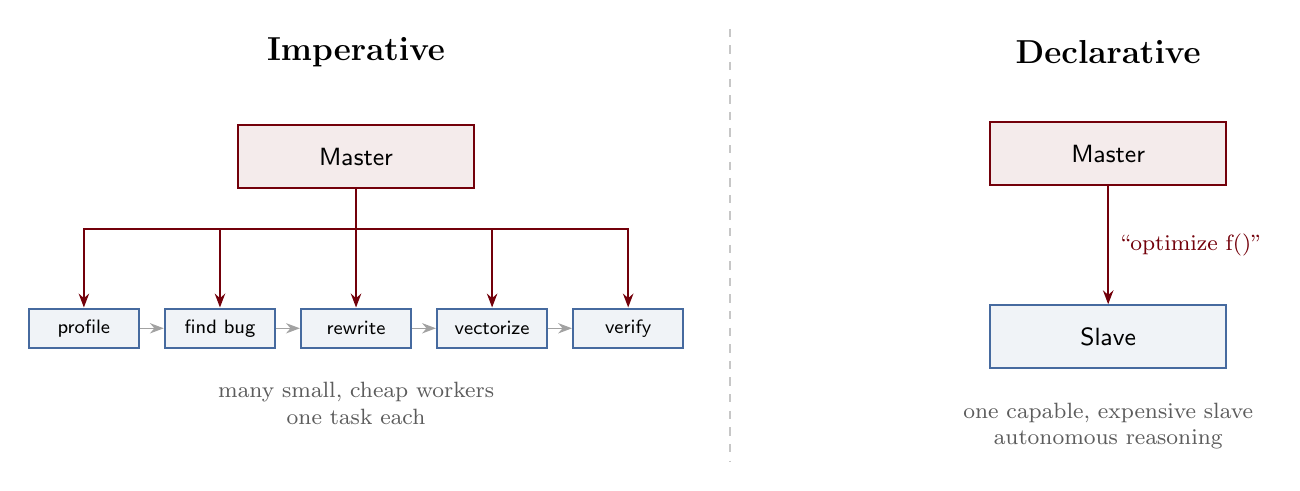
\begin{tikzpicture}[node distance=0.4cm and 0.8cm]
% Imperative
\node[font=\large\bfseries] (imp-title) {Imperative};
\node[agentbox=garnet, below=0.6cm of imp-title, minimum width=3cm] (imp-orch) {Master};
\node[workerbox, below=1.5cm of imp-orch, minimum width=1.4cm, minimum height=0.5cm, font=\scriptsize\sffamily] (iw3) {rewrite};
\node[workerbox, left=0.3cm of iw3, minimum width=1.4cm, minimum height=0.5cm, font=\scriptsize\sffamily] (iw2) {find bug};
\node[workerbox, left=0.3cm of iw2, minimum width=1.4cm, minimum height=0.5cm, font=\scriptsize\sffamily] (iw1) {profile};
\node[workerbox, right=0.3cm of iw3, minimum width=1.4cm, minimum height=0.5cm, font=\scriptsize\sffamily] (iw4) {vectorize};
\node[workerbox, right=0.3cm of iw4, minimum width=1.4cm, minimum height=0.5cm, font=\scriptsize\sffamily] (iw5) {verify};
\draw[dataarrow=garnet] (imp-orch.south) -- ++(0,-0.5) -| (iw1.north);
\draw[dataarrow=garnet] (imp-orch.south) -- ++(0,-0.5) -| (iw2.north);
\draw[dataarrow=garnet] (imp-orch.south) -- ++(0,-0.5) -| (iw3.north);
\draw[dataarrow=garnet] (imp-orch.south) -- ++(0,-0.5) -| (iw4.north);
\draw[dataarrow=garnet] (imp-orch.south) -- ++(0,-0.5) -| (iw5.north);
\draw[dataarrow=bk50, thin] (iw1.east) -- (iw2.west);
\draw[dataarrow=bk50, thin] (iw2.east) -- (iw3.west);
\draw[dataarrow=bk50, thin] (iw3.east) -- (iw4.west);
\draw[dataarrow=bk50, thin] (iw4.east) -- (iw5.west);
\node[labelnode, below=0.3cm of iw3, font=\footnotesize, align=center] {many small, cheap workers\\one task each};

% Declarative
\node[font=\large\bfseries, right=7cm of imp-title] (dec-title) {Declarative};
\node[agentbox=garnet, below=0.6cm of dec-title, minimum width=3cm] (dec-orch) {Master};
\node[agentbox=atlantic, below=1.5cm of dec-orch, minimum width=3cm] (dw1) {Slave};
\draw[dataarrow=garnet] (dec-orch) -- (dw1)
  node[midway, right, font=\footnotesize] {``optimize f()''};
\node[labelnode, below=0.3cm of dw1, font=\footnotesize, align=center] {one capable, expensive slave\\autonomous reasoning};

% Separator
\draw[dashed, bk30, thick] ($(imp-title.east)!0.5!(dec-title.west)$) ++(0,0.3) -- ++(0,-5.5);
\end{tikzpicture}
\end{document}
